\documentclass[a4paper]{article}

\usepackage{parskip} % Package to tweak paragraph skipping
\usepackage{tikz} % Package for drawing
\usepackage{amsmath}
\usepackage{amssymb}
\usepackage{hyperref}
\usepackage{graphicx}
\usepackage{wrapfig}

\usepackage[a4paper,margin=1in]{geometry}
\usepackage{fancyhdr}
\pagestyle{fancy}


\title{EE2012/ST2334 Discussion 2}
\author{Liu Zichen}
\date{20 Feb, 2019}
\begin{document}

\maketitle

\begin{enumerate}

\item
\textbf{[random variable]}
Random variable is a function that maps the sample space to a real value space. 
\[X : S \rightarrow \mathbb { R } \in R _ {X}\]
All the possible real values form a set called "range" $R_{X}$.
Recall the pixel example in discussion 1, if I want a random variable to describe the grey level (use the simple average method: $I _ {grey} = ( R + G + B ) / 3$ ) of a single pixel, what's the range $R _ {X}$?

\item
\textbf{[equivalent events]}
Choose any one pair of equivalent events from (1) and explain. Can you see why their probabilities are equal? 

\item
\textbf{[PMF / PDF]}
For a random variable (remember it's a function) $X$, if its range $R _ {X}$ is finite or countably infinite, we call $X$ \textbf{discrete} RV. On the other hand, if $R_{X}$ is an interval or a collection of intervals, we call $X$ \textbf{continuous} RV.

For discrete RV, we use \textbf{probability mass function (PMF)} to describe the probability distribution of $X$; for continuous, we use \textbf{probability density function (PDF)} to describe the probability distribution of $X$. 

An \textbf{\textit{important}} note is that PMF is a proper probability, but PDF is \textbf{NOT} a proper probability! Can you see why?

\item
\textbf{[CDF]}
$F ( x ) = \operatorname { Pr } ( X \leq x )$. PDF for continuous random variable can be otained by $f ( x ) = \frac { d F ( x ) } { d x }$ is the derivative exists.

\item
\textbf{[Expectation]}
Expectation tells us the average (i.e., expected) value of some function $f(x)$ taking into account the distribution of $x$.
\[
\begin{split}
    E [ f ( x ) ] &= \sum _ { x } f ( x ) p ( x ) \\
    E [ f ( x ) ] &= \int f ( x ) p ( x ) d x
\end{split}
\]
\begin{figure}[h]
    \centering
    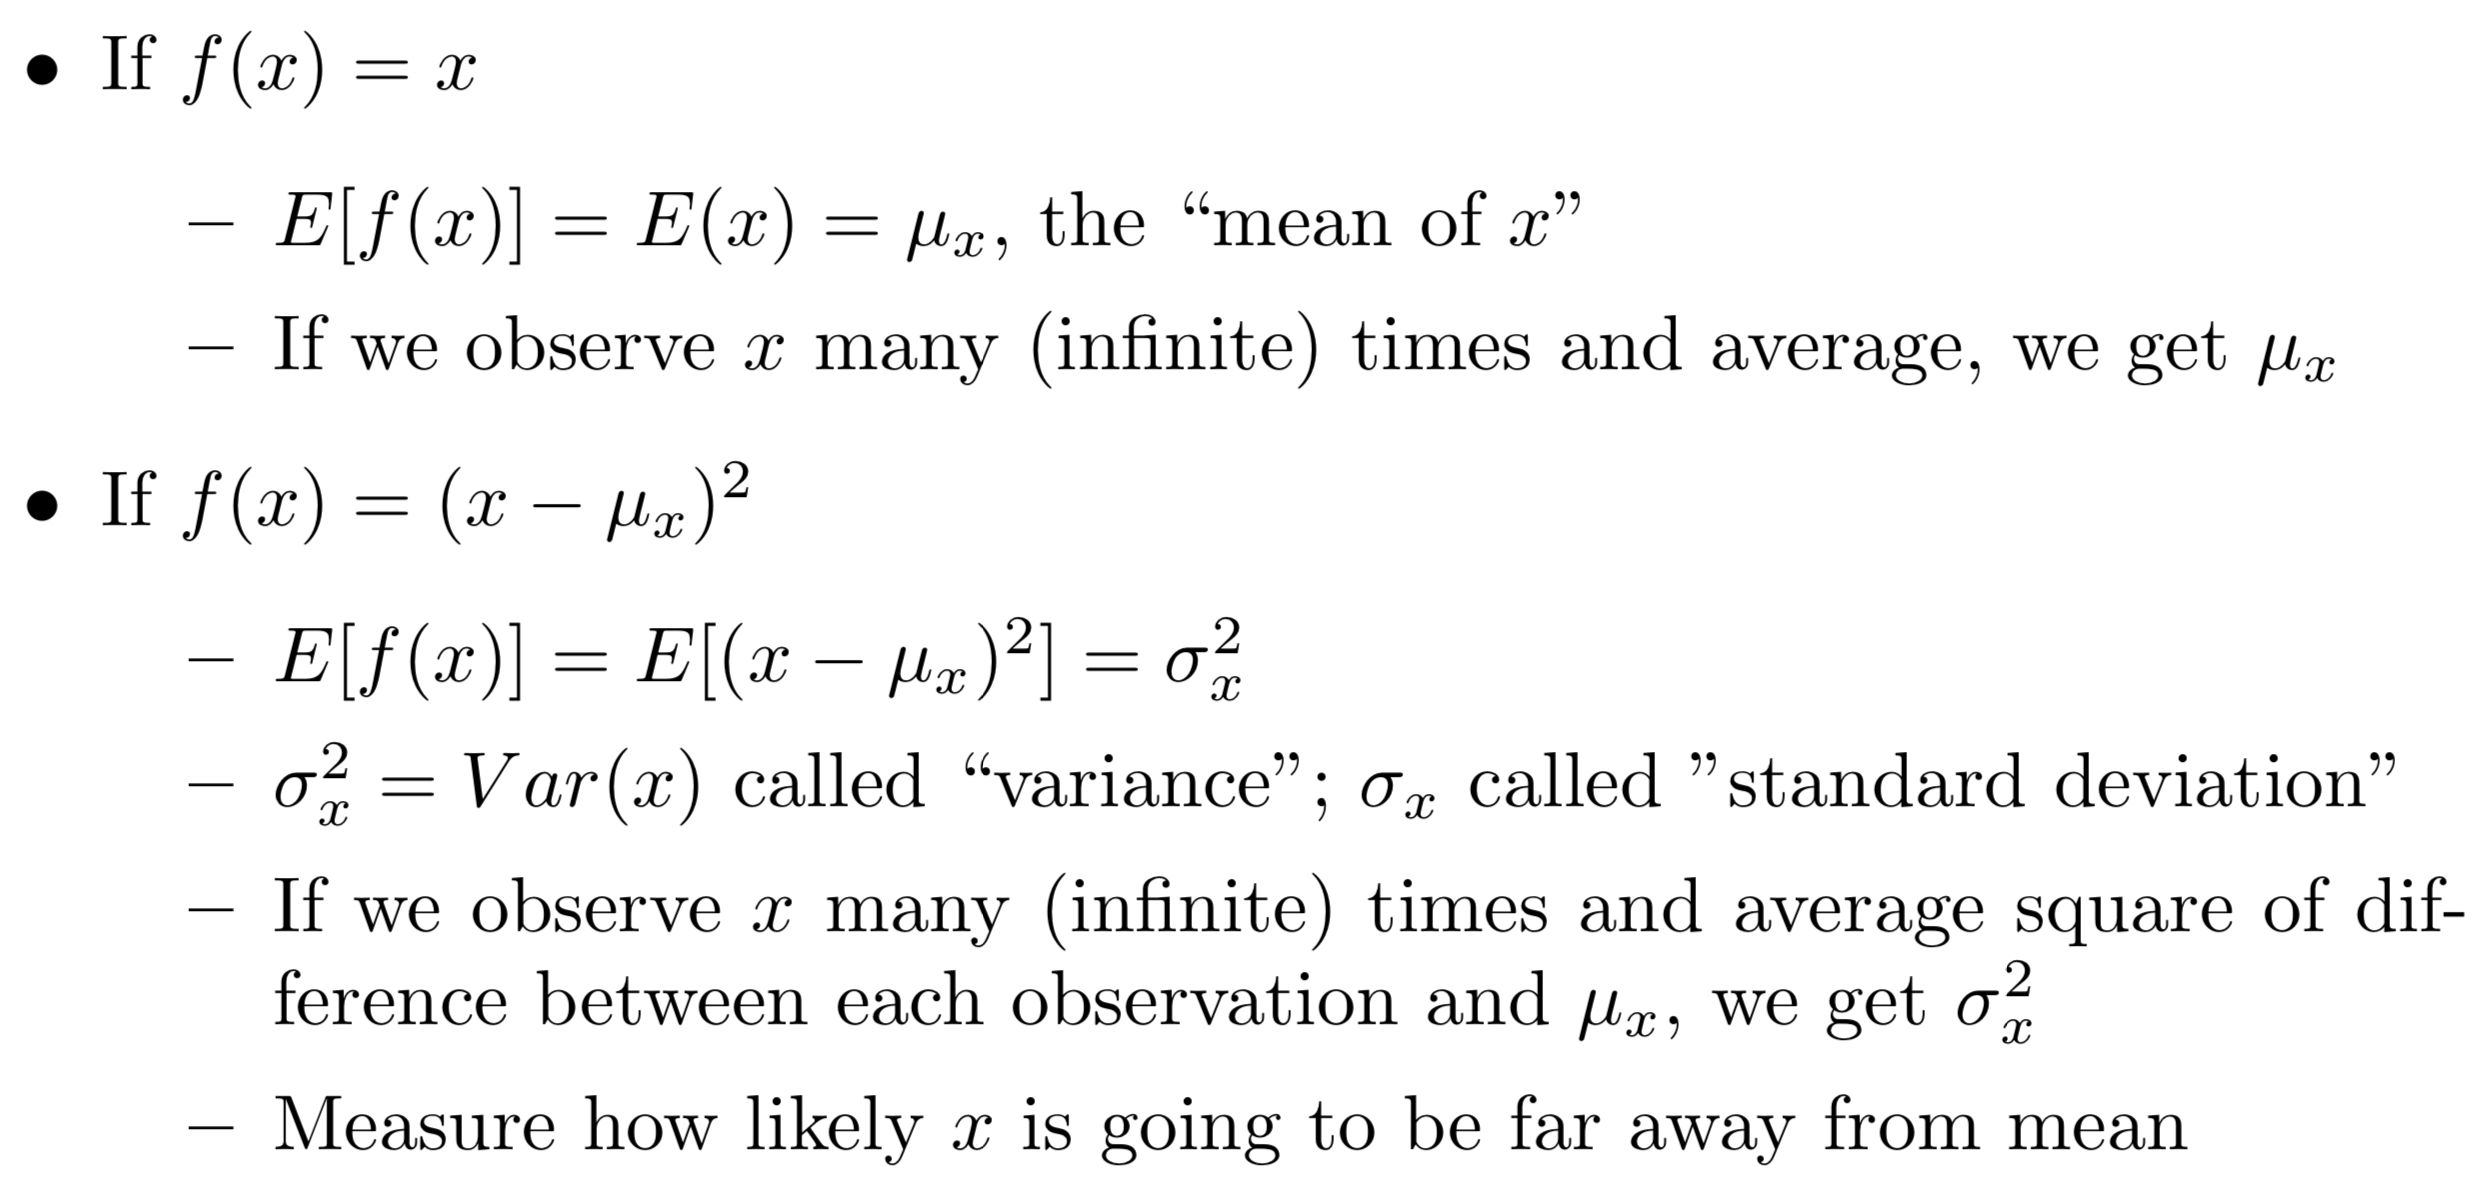
\includegraphics[scale = 0.2]{expectation.png}
\end{figure}

\item
\textbf{[properties]}
For mean: $E ( a X + b ) = a E ( X ) + b$. For variance: $V ( X ) = E \left( X ^ { 2 } \right) - [ E ( X ) ] ^ { 2 }$, $V ( a X + b ) = a ^ { 2 } V ( X )$.

\item
\textbf{[Chebyshev’s Inequality]}
$\operatorname { Pr } ( | X - \mu | > k \sigma ) \leq \frac{1}{ k ^ { 2 }}$, given mean $\mu$ and variance $\sigma$ for a random variable, and $\mathbf{k > 0}$. Another form is $\operatorname { Pr } ( | X - \mu | \leq k \sigma ) \geq 1 - \frac{1}{ k ^ { 2 }}$.

\end{enumerate}
\end{document}